%		For public use only, fair use laws still apply
%		A tutorial template created by Chad Gibbons




%	I recommend for generic help the following website
%	http://www.emerson.emory.edu/services/latex/latex_toc.html
%	There are many good websites and forums for LaTeX
%
%	If you have a problem, google it. (ex. "How do I start my page numbers at a different number")



%%%%%%%%%%%%%%%%%%%%%%%%%%%%%%%%%%%%%%%%%%%%%%%%%%%%%%
%					 													  %
%					 													  %
%					  ALWAYS BEGIN THE PROGRAM WITH								  %
%					 													  %
%						\documentclass{class_type}								  %
%																		  %
%		Different class types have different commands associated with them, similar to header files			  %
%					 													  %
%					 													  %`
%%%%%%%%%%%%%%%%%%%%%%%%%%%%%%%%%%%%%%%%%%%%%%%%%%%%%%

\documentclass[12pt]{article}

%%%%%%%%%%%%%%%%%%%%%%%%%%%%%%%%%%%%%%%%%%%%%%%%%%%%%%
%					 													  %
%					 													  %
%				It is recommended to only use packages as you need them 						  %
%					 													  %
%	Different types of reports will consistently use specific packages; keep these in their respective templates		  %
%					 													  %
%					 													  %
%%%%%%%%%%%%%%%%%%%%%%%%%%%%%%%%%%%%%%%%%%%%%%%%%%%%%%


%\usepackage[a4paper,total={8.27in,11.69in},left=0.56in,right=0.56in,top=0.75in,bottom=1.69in]{geometry}		% 	Margins IEEE Articles
\usepackage[letterpaper,total={8.5in,11in},left=1.25in,top=1in,bottom=1in,right=1in]{geometry}		% 	Margins PDD
%\usepackage[a4paper,total={6.5in,9.375in}]{geometry}		% 	Margins MLA
%\usepackage{babel}				%	Expands text mode
\usepackage[english]{babel}
\usepackage{csquotes}				%	Permits \enquote{quote}
\usepackage{graphicx}				%	Permits \includegraphics[]{image}
\usepackage{caption}				%	Permits the void caption \caption*{}
\usepackage{titlesec}				%	Modify section titles
\usepackage{wrapfig}				% 	Insert wrappable objects like figures or tables
%\usepackage{a4wide}				% 	Expand width of body lazily
\usepackage{multicol}				% 	Permits multicolumn
\usepackage{multirow}				%	Permites utilization of multiple rows of a table
\usepackage{tocloft}				%	Permits modification of Table of Contents
\usepackage{amssymb}				%	Greek Alphabet Symbols
\usepackage{appendix}

\usepackage{scrextend}				% 	Permits padding margins of document


\graphicspath{ {./images/} }			%	Sets filepath to images folder in location of TeX Document

\usepackage[utf8]{inputenc}			%	biblatex depends on on this package
\usepackage{comment}
%\usepackage[backend=bibtex,style=numeric]{biblatex}	%	LaTeX blibliography	%% Note: ieee stle lower-cases titles past first letter (Which seems wrong)
\usepackage[backend=bibtex,style=numeric,sorting=none]{biblatex}
%\bibliographystyle{ieeetr}			% INVESTIGATE FURTHER FOR AUTO ORDERING OF BIB REFERENCES
\bibliography{FDR_Draft}				%	REMEMBER TO RENAME THIS FILE IF MOVING TO NEW .bib


%\addbibresource{hec2.bib}


			%	Makes Table of Contents Functionally a table of Hyperlinks
\usepackage{hyperref}
\hypersetup{
	colorlinks,
	citecolor= black,
	filecolor = black,
	linkcolor = blue,
	urlcolor = blue
	}

			%	Next Three Lines permit use of .tif images in \includegraphics
\usepackage{epstopdf}
\epstopdfDeclareGraphicsRule{.tif}{png}{.png}{convert #1 \OutputFile}
\AppendGraphicsExtensions{.tif}

\renewcommand{\thesection}{\Roman{section}} 
\renewcommand{\thesubsection}{\thesection.\Alph{subsection}}
\renewcommand{\thesubsubsection}{\thesection.\arabic{subsubsection}}
\setlength\cftsecnumwidth{3em}
\setlength\cftsubsecnumwidth{3em}
\setlength\cftsubsubsecnumwidth{3em}

			%	Define Abstract to be IEEE compliant (10pt, centered, roman numerals, capitalized)
\titleformat{\abstract}{\normalfont\btshape}{\Roman{section}}{1em}{\MakeUppercase}
			%	Define Sections to be IEEE compliant (10pt, centered, roman numerals, capitalized)
\titleformat{\section}{\normalfont\filcenter}{\Roman{section}.}{1em}{\MakeUppercase}
			%	Define Subections to be IEEE compliant (10pt, left, roman numerals, capitalized)
\titleformat{\subsection}{\normalfont\itshape}{\Alph{subsection}.}{1em}{}
			%	Define Subsubections to be IEEE compliant (10pt, left, roman numerals, capitalized, inline text)
\titleformat{\subsubsection}[runin]{\normalfont\itshape}{\indent\arabic{subsubsection}.)}{1em}{}
			%	Define Table of Contents to be IEEE compliant


			%	Next Two Lines Make Document San-Serif
%\renewcommand{\familydefault}{\sfdefault}		
%\usepackage{helvet}


\usepackage{textcomp}				%	For subsection symbol w/ \textsection
\usepackage{pdfpages}				%	For inserting PDF document and pages into LaTeX file
							%% 		Recommended pdfpages format : 									%%
							%%		\includepdf[pages=-,width=0.9\linewidth,pagecommand={}]{./appendices/file.pdf}		%%

\newcommand{\cross}[1][1pt]{\ooalign{ 	%	Creating footnote cross symbol
  \rule[1ex]{1ex}{#1}\cr% Horizontal bar
  \hss\rule{#1}{.7em}\hss\cr}}% Vertical bar

%\usepackage[T1]{fontspec}
\usepackage{inconsolata}				%	converts \ttfamily to consolas font
%\IfFileExists{zi4.sty}{\usepackage{zi4}}					%	renamed version of inconsolata
%{\usepackage{inconsolata}}	
%\newfontfamily{\ttconsolas}{Consolas}

  
%%%%%%%%%%%%%%%%%%%%%%%%%%%%%%%%%%%%%%%%%%%%%%%%%%%%%%%			PREAMBLE



%%%%%%%%%%%%%%%%%%%%%%%%%%%%%%%%%%%%%%%%%%%%%%%%%%%%%%%			DOCUMENT




%%%%%%%%%%%%%%%%%%%%%%%%%%%%%%%%%%%%%%%%%%%%%%%%%%%%%%
%					 													  %
%					 													  %
%					  ALWAYS BEGIN THE DOCUMENT WITH								  %
%					 													  %
%							\begin{document}									  %
%					 													  %
%					 													  %
%%%%%%%%%%%%%%%%%%%%%%%%%%%%%%%%%%%%%%%%%%%%%%%%%%%%%%


\begin{document}

\section{Testing and Validation}
\indent
Validation of a product prototype is an important step to determine the performance, reliability, and durability of the designed product. Without proper testing, the product life cycle can be severely limited due to component failure or subcircuit malfunction.  All basic functionality for each subsystem is verified by following standard test practices. The transmitter and receiver subsystems were subjected to validation tests described below to observe their actual performance. 

\pagebreak

\section*{Transmitter Tests} %%%%%%%%%%%%%%%%%%%%%%%%%%%%%%%%%%%%%%%%%%%%%%%%%
\subsection{Transmitter Power Supply Tests}
\indent
The transmitter prototype board testing starts by applying DC voltage on pins 3, and 4 positive terminals and pins 1-7 negative terminals. DC voltage is supplied using a bench power supply with the current limit set to 0.3A. The power supply voltage is gradually increased from 0V to the nominal voltage of 48V while the bench power supply current was constantly monitored.
The 30V regulator will start regulating if the input voltage is higher than 38.3V. The expected output voltage on TP 1 is 30V +/-2\% due to reference voltage tolerance and resistors used for setting the output voltage.\\

\noindent
After the 30V regulator test, the voltage output is verified the following low voltage regulators are verified:\\
\hfill \\
\indent \indent $\cdot$ 3.3V regulator (U11) test point TP2 nominal voltage 3.3V  tolerance +/- 1.5\% \\
\indent \indent $\cdot$ 5V regulator (U11) test point TP3 nominal voltage 5V  tolerance +/- 1.5\%\\

\noindent
Below is the part of the schematic diagram showing test points TP1, TP2, and TP3.
\hfill
\begin{figure}[h!]
\centering
\includegraphics[width=0.82\linewidth]{Transmitter_power_supply_sch_diag}
\caption{Transmitter Voltage Regulator Circuits}
\end{figure}

\hfill \\
\indent
After power modules are verified the test firmware can be loaded using a JTAG connection on the board.  The firmware sets all parameters in the default state for testing. The coil driver is disabled and all peripherals are turned off.

\subsection{Transmitter Coil Driver Tests}
\indent
After the firmware is loaded the board is turned off and the transmitter coil is connected to the terminals J3 and J4. The coil driver circuit is tested using a variable voltage supply. To perform this test PPTC fuse, F1 is removed and the bench power supply is connected to the TP1 (positive terminal) and the negative terminal is connected to the ground.  The oscilloscope probe is attached to the drain of  Q1 (GaN FET transistor).  The second probe is connected to the output of the 13.56MHz temperature compensated oscillator (TP4).\\

\indent
After the test equipment is attached the power supply is turned on and the output voltage is gradually increased. When the power supply is higher than 5V voltage regulators (3.3V and 5V) are enabled and they provide power to the transmitter subcircuits.  The temperature compensated oscillator (TXCO) enable line is controlled by push buttons. When the oscillator enable line is set to a high level a 13.56MHz signal is enabled and 13.56MHz is fed into the Class E amplifier driver (U11). The expected voltage from the TXCO on TP4 is 3.3Vpp.  After the oscillator subcircuit is verified the oscilloscope probe is placed on one of the terminals of jumper R32 to verify the functionality of U11. The expected amplitude on the output of the Class E amplifier driver is 5Vpp.\\

\noindent
The figure below presents the subcircuit wherein the transmission signal is generated and tested.
\hfill
\begin{figure}[h!]
\centering
\includegraphics[width=0.9\linewidth]{TX_oscillator_and_buffer}
\caption{Oscillator and Buffer Subcircuit}
\end{figure}
\hfill \\
\pagebreak

\indent
The GaN FET switching is verified by observing the GaN FET drain voltage waveform that will have a voltage swing from 0V to 117V if the power supply voltage is set to 30 V. For lower supply voltages the swing will be lower but it always should swing from 0V to some positive voltage.  After the GaN FET switching is verified the transmitter coil resonance will be adjusted. \\

\indent
To set transmitter coil resonance a variable capacitor (C28) must be adjusted while the voltage across the coil is monitored using a 100X oscilloscope probe attached to J4  (transmitter board coil terminal). The trimmer capacitor must be adjusted until the voltage across the transmitter coil reaches the maximum value. After the resonance is achieved the power supply voltage is gradually increased to 30V while the supply current is constantly monitored.  The expected voltage on the drain of the GaN FET is 117Vpp. The measured voltage is recorded.  The 30V power supply current should be 120mA if there is no load present (no receiver coil in the front of the transmitter coil).\\

\noindent
The figure below presents the subcircuit wherein the transmission signal is amplified and observed by a Class E amplifier.
\hfill
\begin{figure}[h!]
\centering
\includegraphics[width=0.9\linewidth]{Class_E_amplifier}
\caption{Transmission Signal Class E Amplifier Subcircuit}
\end{figure}
\hfill \\
\pagebreak
\hfill \\
\indent
Transmitter power output is measured when the class E amplifier is verified and the amplifier power supply voltage is 30V.  The specified transmitter power output is 30W. The power output is measured by placing receiving LC circuit loaded with a 50Ω high power resistor in the front of the transmitter coil at a distance of 5 cm. The peak to peak voltage across the load is measured using the oscilloscope and recorded in the table. This process is repeated for distances of 4 cm, 3 cm, 2 cm, and 1 cm.
\hfill
\begin{figure}[h!]
\centering
\includegraphics[width=0.75\linewidth]{Variable_RX-TX_Distance}
\caption{Received Power vs. Distance Test Setup}
\end{figure}

\subsection{Transmitter Firmware Tests}

\noindent
The figure below is a reference for the transmitter part numbers and pin numbers.  The part numbers can be found adjacent to the part outline with a prefix of P, J, U, Q, F, D, R, C, or L.  Pin numbers are found without a prefix adjacent to the first and last pin with their respective number in any part denoted by the prefix P where space provides.
\hfill
\begin{figure}[h!]
\centering
\includegraphics[width=0.8\linewidth]{receiver_pcb_layout}
\caption{Reference Layout for Part and Pin Numbers}
\end{figure}

\hfill
\pagebreak
\hfill 
\subsection{Transmitter Firmware Tests}

\indent
The first recommendation in any trouble rise of troubleshooting of quality assurance is to check the mcu\_setup.c and mcu\_setup.h files.  Additionally, it is good to note that a unit test is a type of software test that only requires building a small portion of the codebase in order to test a set of specific modules.  Unit testing reduces the total amount of time dedicated into the development of any software.

%%% Currently at once every two seconds
\subsubsection*{The MCU Clock On LED} (MCU\_Clock\_on or D8 by the microcontroller) should be blinking at a rate of approximately twice every second \textbf{(This rate is subject to change)}.  If this is not occurring, the clock interrupt routine is not operating properly.  Investigate for over-polling at the UART RX Pins (P2.0 and P2.5) is occurring.  Alternatively, the TX Pins could be written out of turn (P2.1 and P2.6) which would thus initiate the UART Interrupts EUSCI\_A0\_VECTOR (located at P2.0 and P2.1) or EUSCI\_A1\_VECTOR (located at P2.5 and P2.6).  If this is not the case, the next step would be to troubleshoot the ADC (Analog to Digital Converter) Pins (P3.0, P3.1, P3.2, and P3.3).  If this issue where the ADC12\_B\_VECTOR interrupt contravenes the clock interrupt is detected, the error is likely caused by a breakdown in the hierarchy of interrupts.  In such a case, the code must be provided additional logic on how to handle specific interrupts in the scheduler’s run method.

\subsubsection*{The LCD Ticker Panel} should display some coherent statement or acronym.  If it does not, running of a “Hello World” unit test to the LCD is required for appropriate troubleshooting.  The unit test should utilize the identical function used in the production code.  If the unit test passes without errors, the error would reside in the accumulation of text that is meant to be passed into the LCD Ticker Panel.

\subsubsection*{The UART (RX/TX) CON} tests require unit tests. There are four unit tests to be done to test the non-Bluetooth UART ports (P2.5 and P2.6).  The first involves transmitting a ‘A’ character to the same PCB’s RX\_CON Pin (P2.5).  The next unit test would involve transmitting a string and acknowledgement TCP handshake.  These same unit tests are repeated with a secondary PCB.

\subsubsection*{The Bluetooth} validation tests will involve a unit test from the personal computer that connects to the receiver and sweeps through a set of pre-programmed unit tests that provide specific responses and sample data points.

\subsubsection*{The Wireless Power Transmission (WPT) Signal Generation} test should be conducted prior to connecting the transmitter's WPT coil.  Press Button 0 at SW1 to turn on the signal generator and measure the voltage at the transmitter WPT Coil Junction points (J3 with J4 as well as J5 with J6).  Once the voltage is observed, press Button 1 at SW2 to turn off the signal generator, and a drop off of voltage should be observed. \textbf{(NOTE: The button closest to the microcontroller is Button 0 while the button furthest from the microcontroller and closest to the pins of Part P5 is Button 4. The buttons are arranged in sequential order.)}
%%%%%%%%%%%%%%%  NEED WPT_PEAK_DETECTOR Algorithm
\hfill
\pagebreak
\section*{Receiver Tests}  %%%%%%%%%%%%%%%%%%%%%%%%%%%%%%%%%%%%%%%%%%%%

\subsection{Receiver Power Supply Tests}
\indent
The receiver prototype board testing starts by applying DC voltage across coil terminals for power supply verification at the Receiver Coil Junction Points (J2 and J4).  The Coil terminal subcircuit is shown in the figure below.
\hfill
\begin{figure}[h!]
\centering
\includegraphics[width=0.75\linewidth]{RX_COIL_TERMINALS}
\caption{Receiver Coil Terminal Subcircuit}
\end{figure}
\hfill \\
\indent
This test is necessary for determining whether the voltage regulators output voltages are matching the design specification.\\

\noindent
The following voltage regulators are verified in this test:
\indent \indent $\cdot$3.3V regulator (U12) test point TP2 nominal voltage 3.3V  tolerance +/- 1.5\%\\
\indent \indent $\cdot$5V regulator (U11) test point TP1 nominal voltage 5V  tolerance +/- 1.5\%\\
\indent \indent $\cdot$18V regulator (U13A) test point TP3 nominal voltage 18V tolerance +/- 2\%\\

\noindent
After power module verification the test firmware can be loaded using a JTAG connection on the board.  The firmware sets all parameters in the default state for testing.

\hfill \\
\pagebreak

\subsection{Receiver Wireless Power Rectifier Tests}

\noindent
Specification  for AC-DC (RF-DC) conversion efficiency is 80\%\\
 
\noindent
Conversion efficiency is tested using resistive load and without any other circuit attached to the DC side of the converter (R43 is removed). The load voltage and current are continuously  measured.  The specified receiver coil distance from the charger coil is 5 cm max.
\subsubsection*{Efficiency Test Protocol}\hfill \\
\noindent
This test is determines the efficiency of the power transfer at various distances:\\
\indent \indent $\cdot$The transmitter RF output is set to output 30W.\\
\indent \indent $\cdot$The receiver coil is placed at a 5 cm distance from the transmitter\\
\indent \indent $\cdot$Current and load voltage are recorded\\

\noindent
Previous steps are performed for distances 4 cm, 3 cm 2 cm, and 1 cm.  Using collected information load power is calculated.  Efficiency is calculated using the following equation:

\begin{equation}
\eta = \frac{P_{receiver}}{P_{transmitter}} \cdot 100\%
\end{equation}
\hfill
\begin{figure}[h!]
\centering
\includegraphics[width=0.8\linewidth]{RX_EFF_TEST}
\caption{Receiver RF-DC Converter Efficiency Test Setup}
\end{figure}

\subsection{Receiver Battery Charger Tests}

\indent
The bench power supply current should initially be llimited to 1A and the initial voltage should be set to 20V.  There are two diode voltage drops (1.4V) in the full wave rectifier bridge circuit.  18.6V on charger input is high enough for the proper operating voltage for the LTC4162-L battery charger.  The charger is functional without the battery pack and according to the datasheet, the voltage on the charger output will rise to the programmed constant-voltage value. By measuring this voltage it is possible to determine whether the charger regulates the proper voltage for a given programmed value.
\hfill 
\pagebreak
\hfill \\

\indent
A 18650 battery with two cells in series discharged to 3.2-3.8V per cell may be used for constant current and constant voltage charge testing.  The bench power supply should be connected followed by the battery and no change in MCU behavior should be noted. Constant current charging should begin.  The current limit of the bench power supply may be increased and the charging current should increase up to a maximum of 3.2A. The maximum charging current, charging voltage, cell count, and power supply current and voltage should be recorded and efficiency calculated.\\

\indent Then the power supply should be disconnected and reconnected and there should be no effect on the MCU power state. Charging should automatically resume when the power supply is reconnected. The battery should be allowed to charge until it enters constant voltage mode, which may be recognized by a slowly decreasing charge current that is much lower than the maximum current observed during constant current charging.  A 2 ohm load should be connected to the battery under charge for at least 30 seconds and removed without any effect on MCU operation.

\subsection{Receiver Firmware Tests}

\indent
The first recommendation in any trouble rise of troubleshooting of quality assurance is to check the mcu\_setup.c and mcu\_setup.h files.  Additionally, it is good to note that a unit test is a type of software test that only requires building a small portion of the codebase in order to test a set of specific modules.  Unit testing reduces the total amount of time dedicated into the development of any software.

%%% Currently at once every two seconds
\subsubsection*{The MCU Clock On LED} (MCU\_Clock\_on or D8 by the microcontroller) should be blinking at a rate of approximately twice every second \textbf{(This rate is subject to change)}.  If this is not occurring, the clock interrupt routine is not operating properly.  Investigate for over-polling at the UART RX Pins (P2.0 and P2.5) is occurring.  Alternatively, the TX Pins could be written out of turn (P2.1 and P2.6) which would thus initiate the UART Interrupts EUSCI\_A0\_VECTOR (located at P2.0 and P2.1) or EUSCI\_A1\_VECTOR (located at P2.5 and P2.6).  If this is not the case, the next step would be to troubleshoot the ADC (Analog to Digital Converter) Pins (P3.0, P3.1, P3.2, and P3.3).  If this issue where the ADC12\_B\_VECTOR interrupt contravenes the clock interrupt is detected, the error is likely caused by a breakdown in the hierarchy of interrupts.  In such a case, the code must be provided additional logic on how to handle specific interrupts in the scheduler’s run method.

\subsubsection*{The LCD Ticker Panel} should display some coherent statement or acronym.  If it does not, running of a “Hello World” unit test to the LCD is required for appropriate troubleshooting.  The unit test should utilize the identical function used in the production code.  If the unit test passes without errors, the error would reside in the accumulation of text that is meant to be passed into the LCD Ticker Panel.

\subsubsection*{The UART (RX/TX) CON} tests require unit tests. There are four unit tests to be done to test the non-Bluetooth UART ports (P2.5 and P2.6).  The first involves transmitting a ‘A’ character to the same PCB’s RX\_CON Pin (P2.5).  The next unit test would involve transmitting a string and acknowledgement TCP handshake.  These same unit tests are repeated with a secondary PCB.

\subsubsection*{The Bluetooth} validation tests will involve a unit test from the personal computer that connects to the receiver and sweeps through a set of pre-programmed unit tests that provide specific responses and sample data points.  The Bluetooth tests for the receiver should also include data requests pertaining to the voltage from the battery, the battery's current charge, and any data utilized in the battery charger.
\hfill \\
\pagebreak
\hfill
\section*{System Tests}
\subsection{Coil Test}
Coil impedance is measured using Vector Network Analyzer (VNA). The impedance measurement is obtained by setting the instrument to measure S-parameters (S11) at 13.56 MHz.  Before measurements, the instrument must be calibrated using calibration standards (short circuit, open circuit, and 50$\omega$ load).  The measured impedance is in complex form R+jX form.\\

\noindent
Specified inductance: 909.66nH\\

\noindent
The coil's inductance is determined using the formula below:
\begin{equation}
L = \frac{X_L}{\omega}
\end{equation}
\noindent
Where $\omega$ = 2$\pi$f\\

\noindent
The figure below shows the the equivalent circuit of how the transmitter / receiver coils were evaluated using a Vector Network Analyzer.
\hfill
\begin{figure}[h!]
\centering
\includegraphics[width=0.5\linewidth]{RX_SUBSYSTEM_COIL_TERMINALS.PNG}
\caption{VNA Test Setup}
\end{figure}

\pagebreak

\noindent
Although VNA is not very precise for quality factor measurements it still can be used for estimation. The quality factor is determined by obtaining S21 parameter (forward voltage gain).\\

\noindent
Specified Q factor: 1119\\
 
 \noindent
The quality factor also can be determined by dividing reactance by the resistance the formula is shown below:
\begin{equation}
Q = \frac{X_L}{R}
\end{equation}

\subsection{System Level Firmware Tests}

\subsubsection*{The Bluetooth Localization Test} utilizes the “M” command on the RN4870 BLE chip with 3 prior locations to triangulate which direction is moving towards the transmitter.  This test begins with a computer provided unit test that accepts four distances, the first three that are used to triangulate the receiver in reference to the transmitter and a fourth that must be closer than all three triangulating distances to be considered passing.
\hfill 
\pagebreak

\subsection{Test Results Summary}

\subsubsection{Transmitter Evaluations} \hfill
\subsubsection*{DC Power Test} \hfill \\
\noindent
30V regulator no-load condition measured output voltage 30.04 V\\
5V regulator measured output voltage TP3 5.03V\\
3.3V regulator measured output voltage TP2 3.33V\\
 
\subsubsection*{Coil Driver Test} \hfill \\
Oscillator output voltage TP4 3.69V$_{pp}$\\
 
\noindent
Oscillator output Frequency (13.56 MHz) measured: 13.56MHz\\
Class E amplifier driver voltage jumper R32 (nominal 5Vpp) measured 5.80Vpp
\hfill
\begin{figure}[h!]
\centering
\includegraphics[width=0.8\linewidth]{osc_out}
\caption{Class E Amplifier Driver Output}
\end{figure}
\hfill \\
\pagebreak

\noindent
Q1 Dran nom. 117 V$_{pp}$ (30 V supply) Measured 102V$_{pp}$
\hfill
\begin{figure}[h!]
\centering
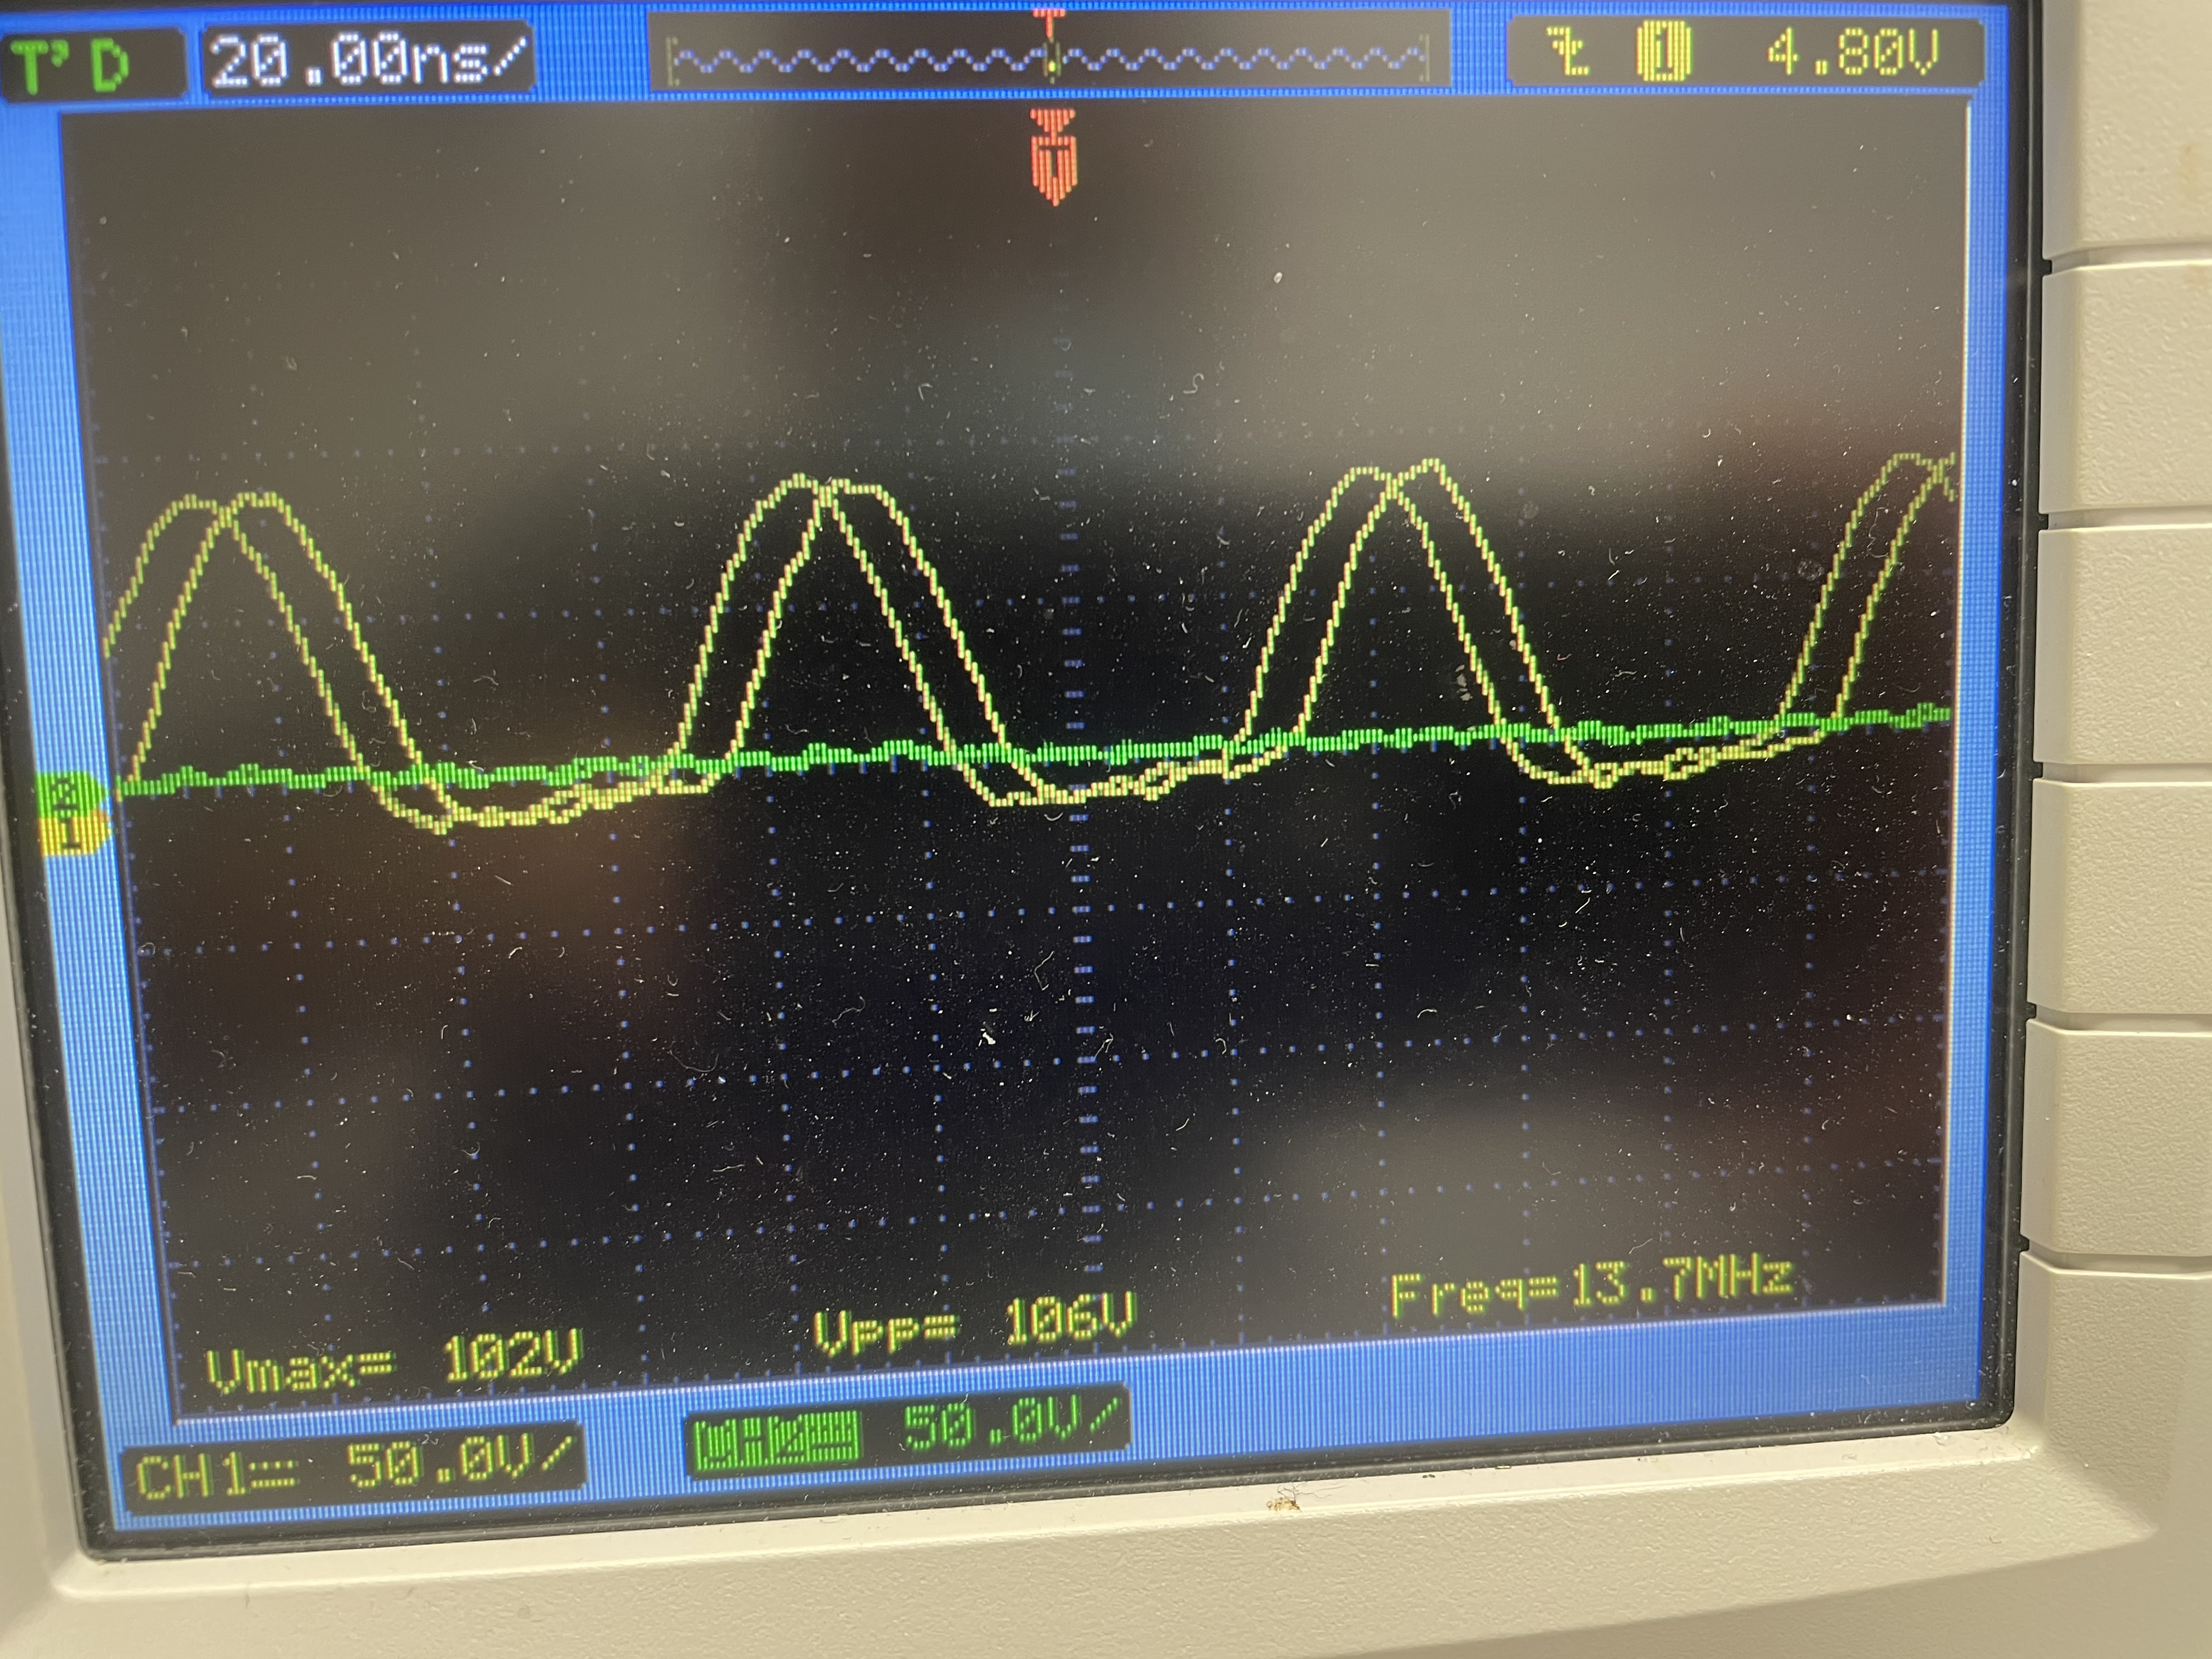
\includegraphics[width=0.65\linewidth]{Q1_measured}
\caption{Q1 Drain Voltage Waveform}
\end{figure}

\noindent
Transmitter coil voltage 117 V$_{pp}$ (30 V supply) Measured 204V$_{pp}$
\hfill
\begin{figure}[h!]
\centering
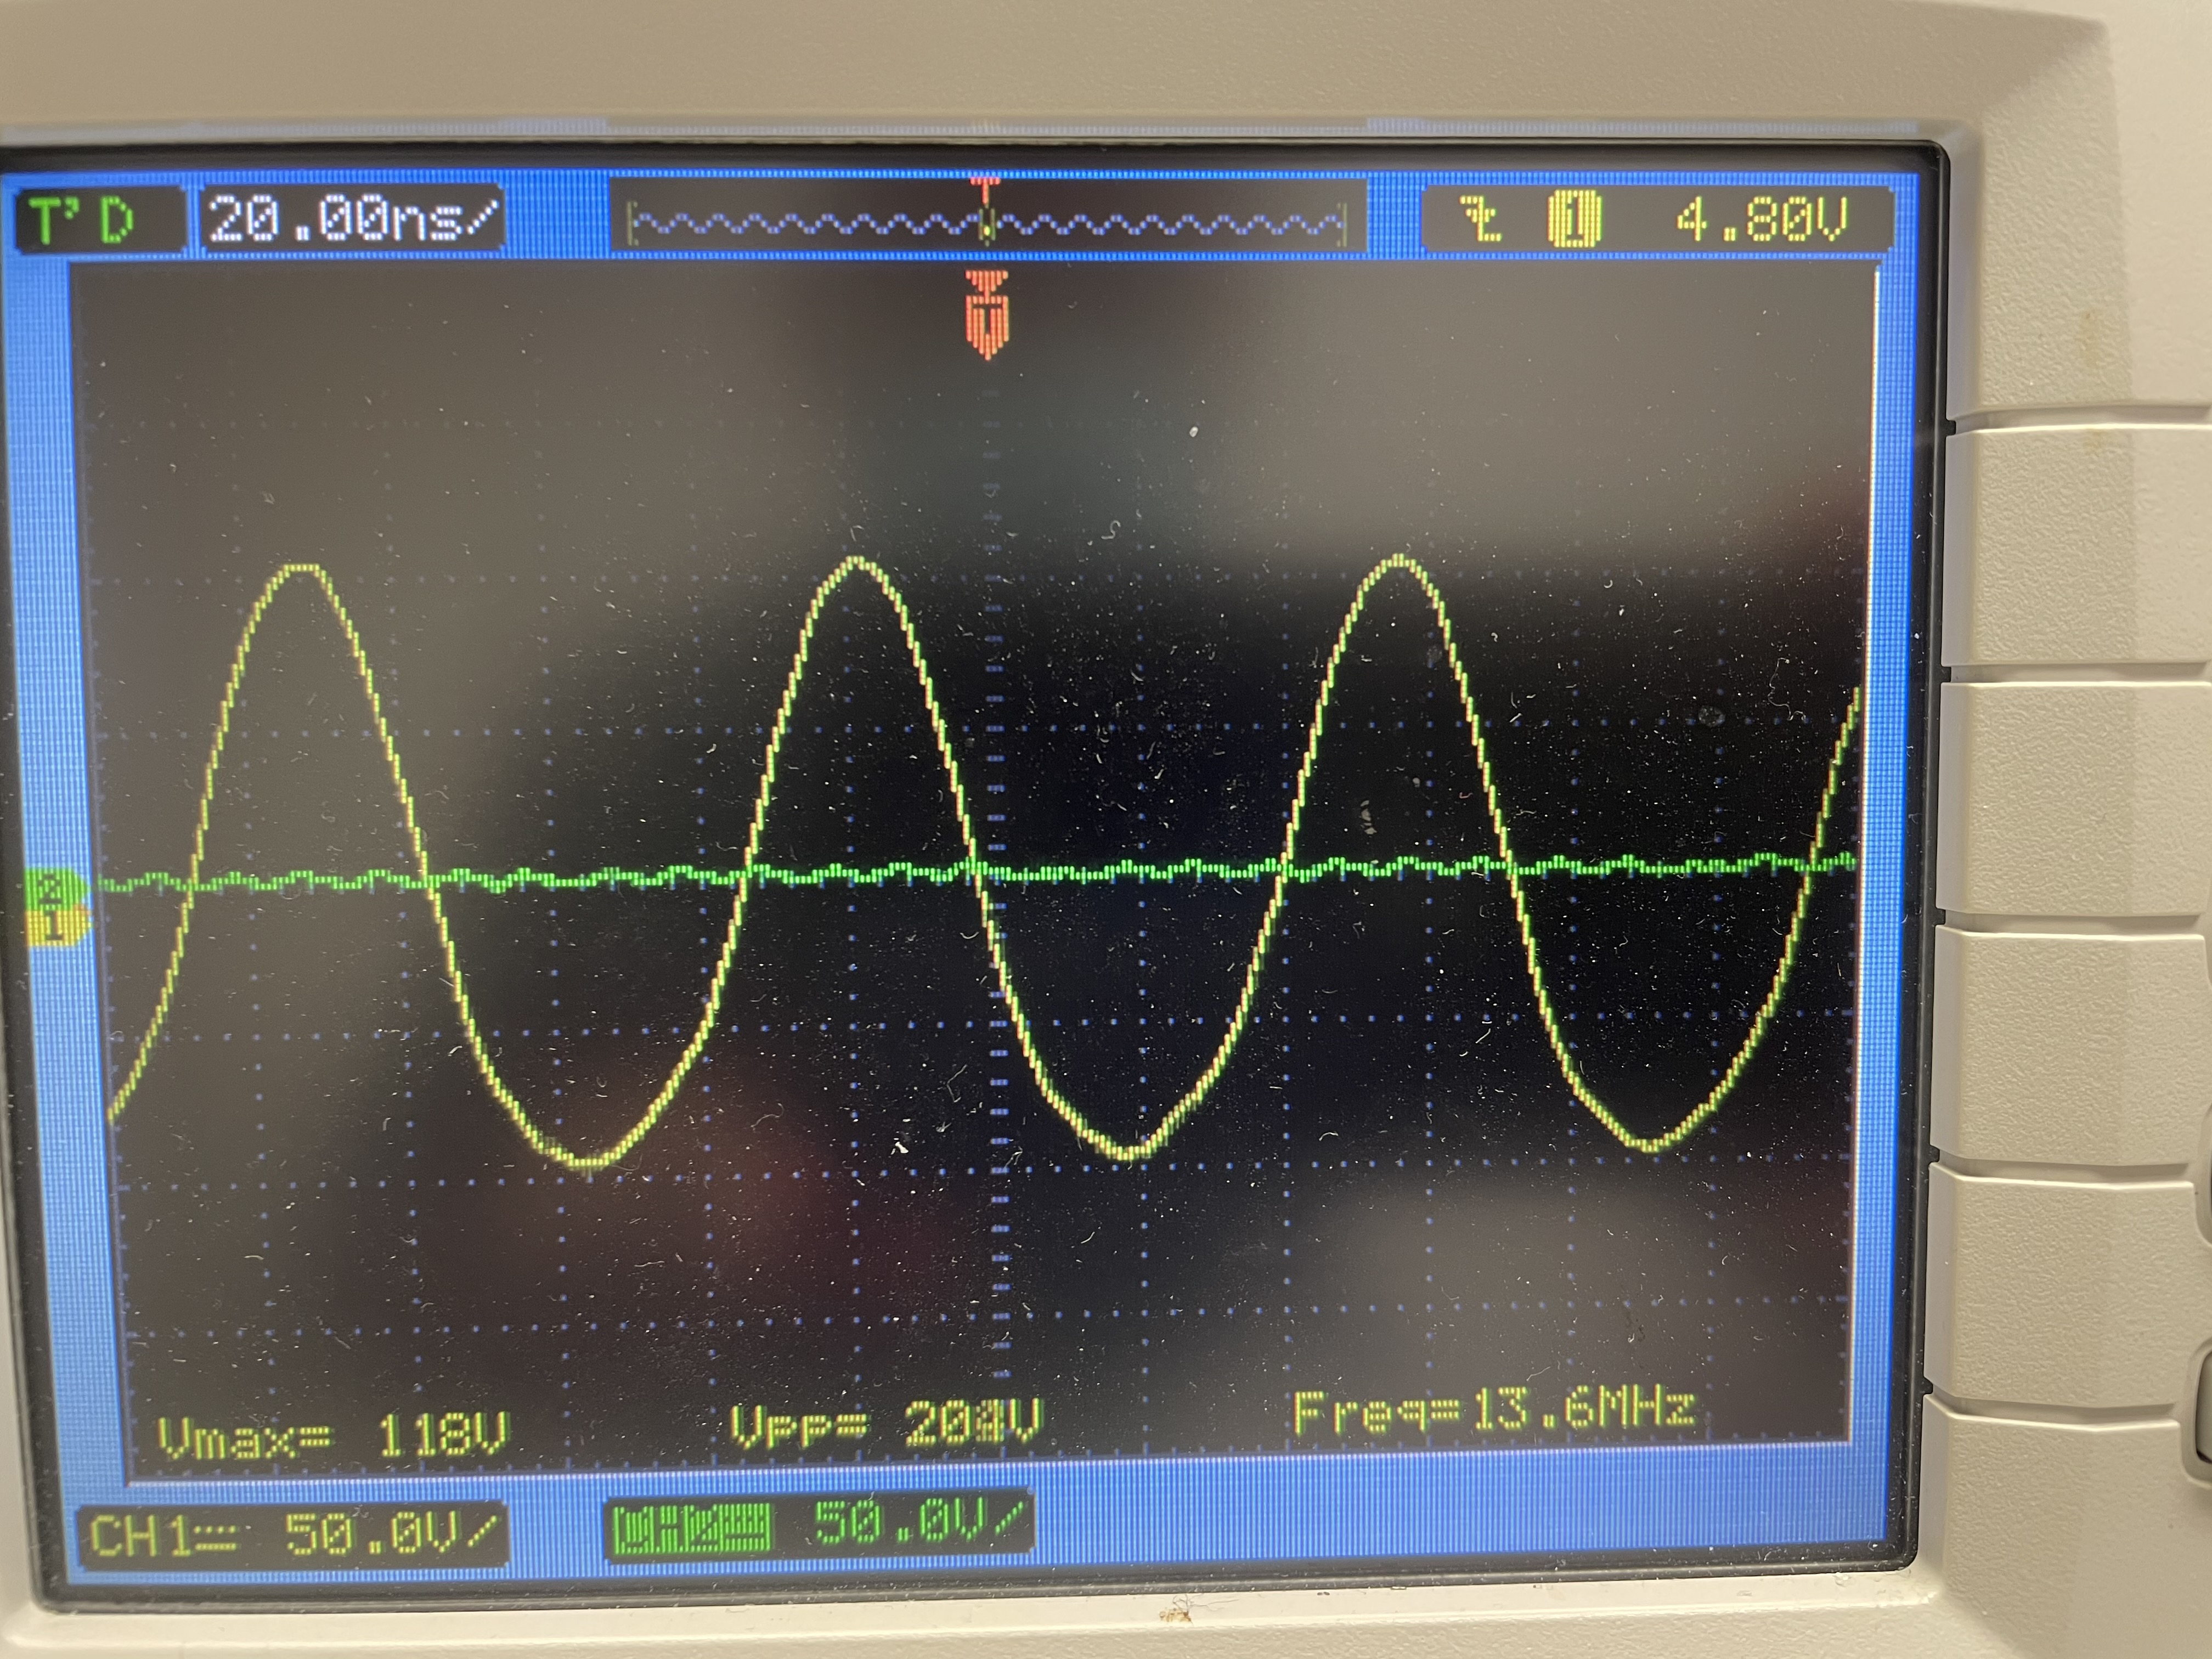
\includegraphics[width=0.65\linewidth]{t_coil_v_measured}
\caption{Q1 Drain Voltage Waveform}
\end{figure}
\hfill 
\pagebreak
\hfill \\
\noindent
Transmitter subsystem input current at 30V supply (120 mA nom. no laod) Measured 140 mA

\begin{table}[h!]
\centering
%Received Power (DC) vs Distance Test
\caption{Transmitted Power vs. Distance Test}
\begin{tabular}{ | c | c | c | }
\hline
 Distance [cm] & Measured Voltage [V$_{pp}$] & Received Power [W] \\
 \hline
5 & & \\
\hline
4 & & \\
\hline
3 & & \\
\hline
2 & & \\
\hline
1 & & \\
\hline
\end{tabular}
\end{table}

\subsubsection{Receiver Evaluations} \hfill \\
\subsubsection*{DC Power Test} \hfill \\
\noindent
5V regulator measured output voltage TP1 5.07V\\
3.3V regulator measured output voltage TP2 3.33V\\
18V regulator measured output voltage TP3 18.26V\\

\begin{table}[h!]
\centering
\caption{Received Power (DC) vs Distance Test}
\begin{tabular}{ | c | c | c |  c |}
\hline
Distance [cm] & Measured Voltage [V] & Measured Current [A] & Power Received [W] \\
\hline
5 & & & \\
\hline
4 & & & \\
\hline
3 & & & \\
\hline
2 & & & \\
\hline
1 & & & \\
\hline
\end{tabular}
\end{table}

\subsubsection*{Coil Design Verification Test}\hfill \\
\noindent
Specified inductance: 909.66nH\\ 
Measured impedance at 13.56MHz: 0.43 +j78.28$\Omega$\\
\hfill \\
\pagebreak
\hfill \\
\begin{figure}[h!]
\centering
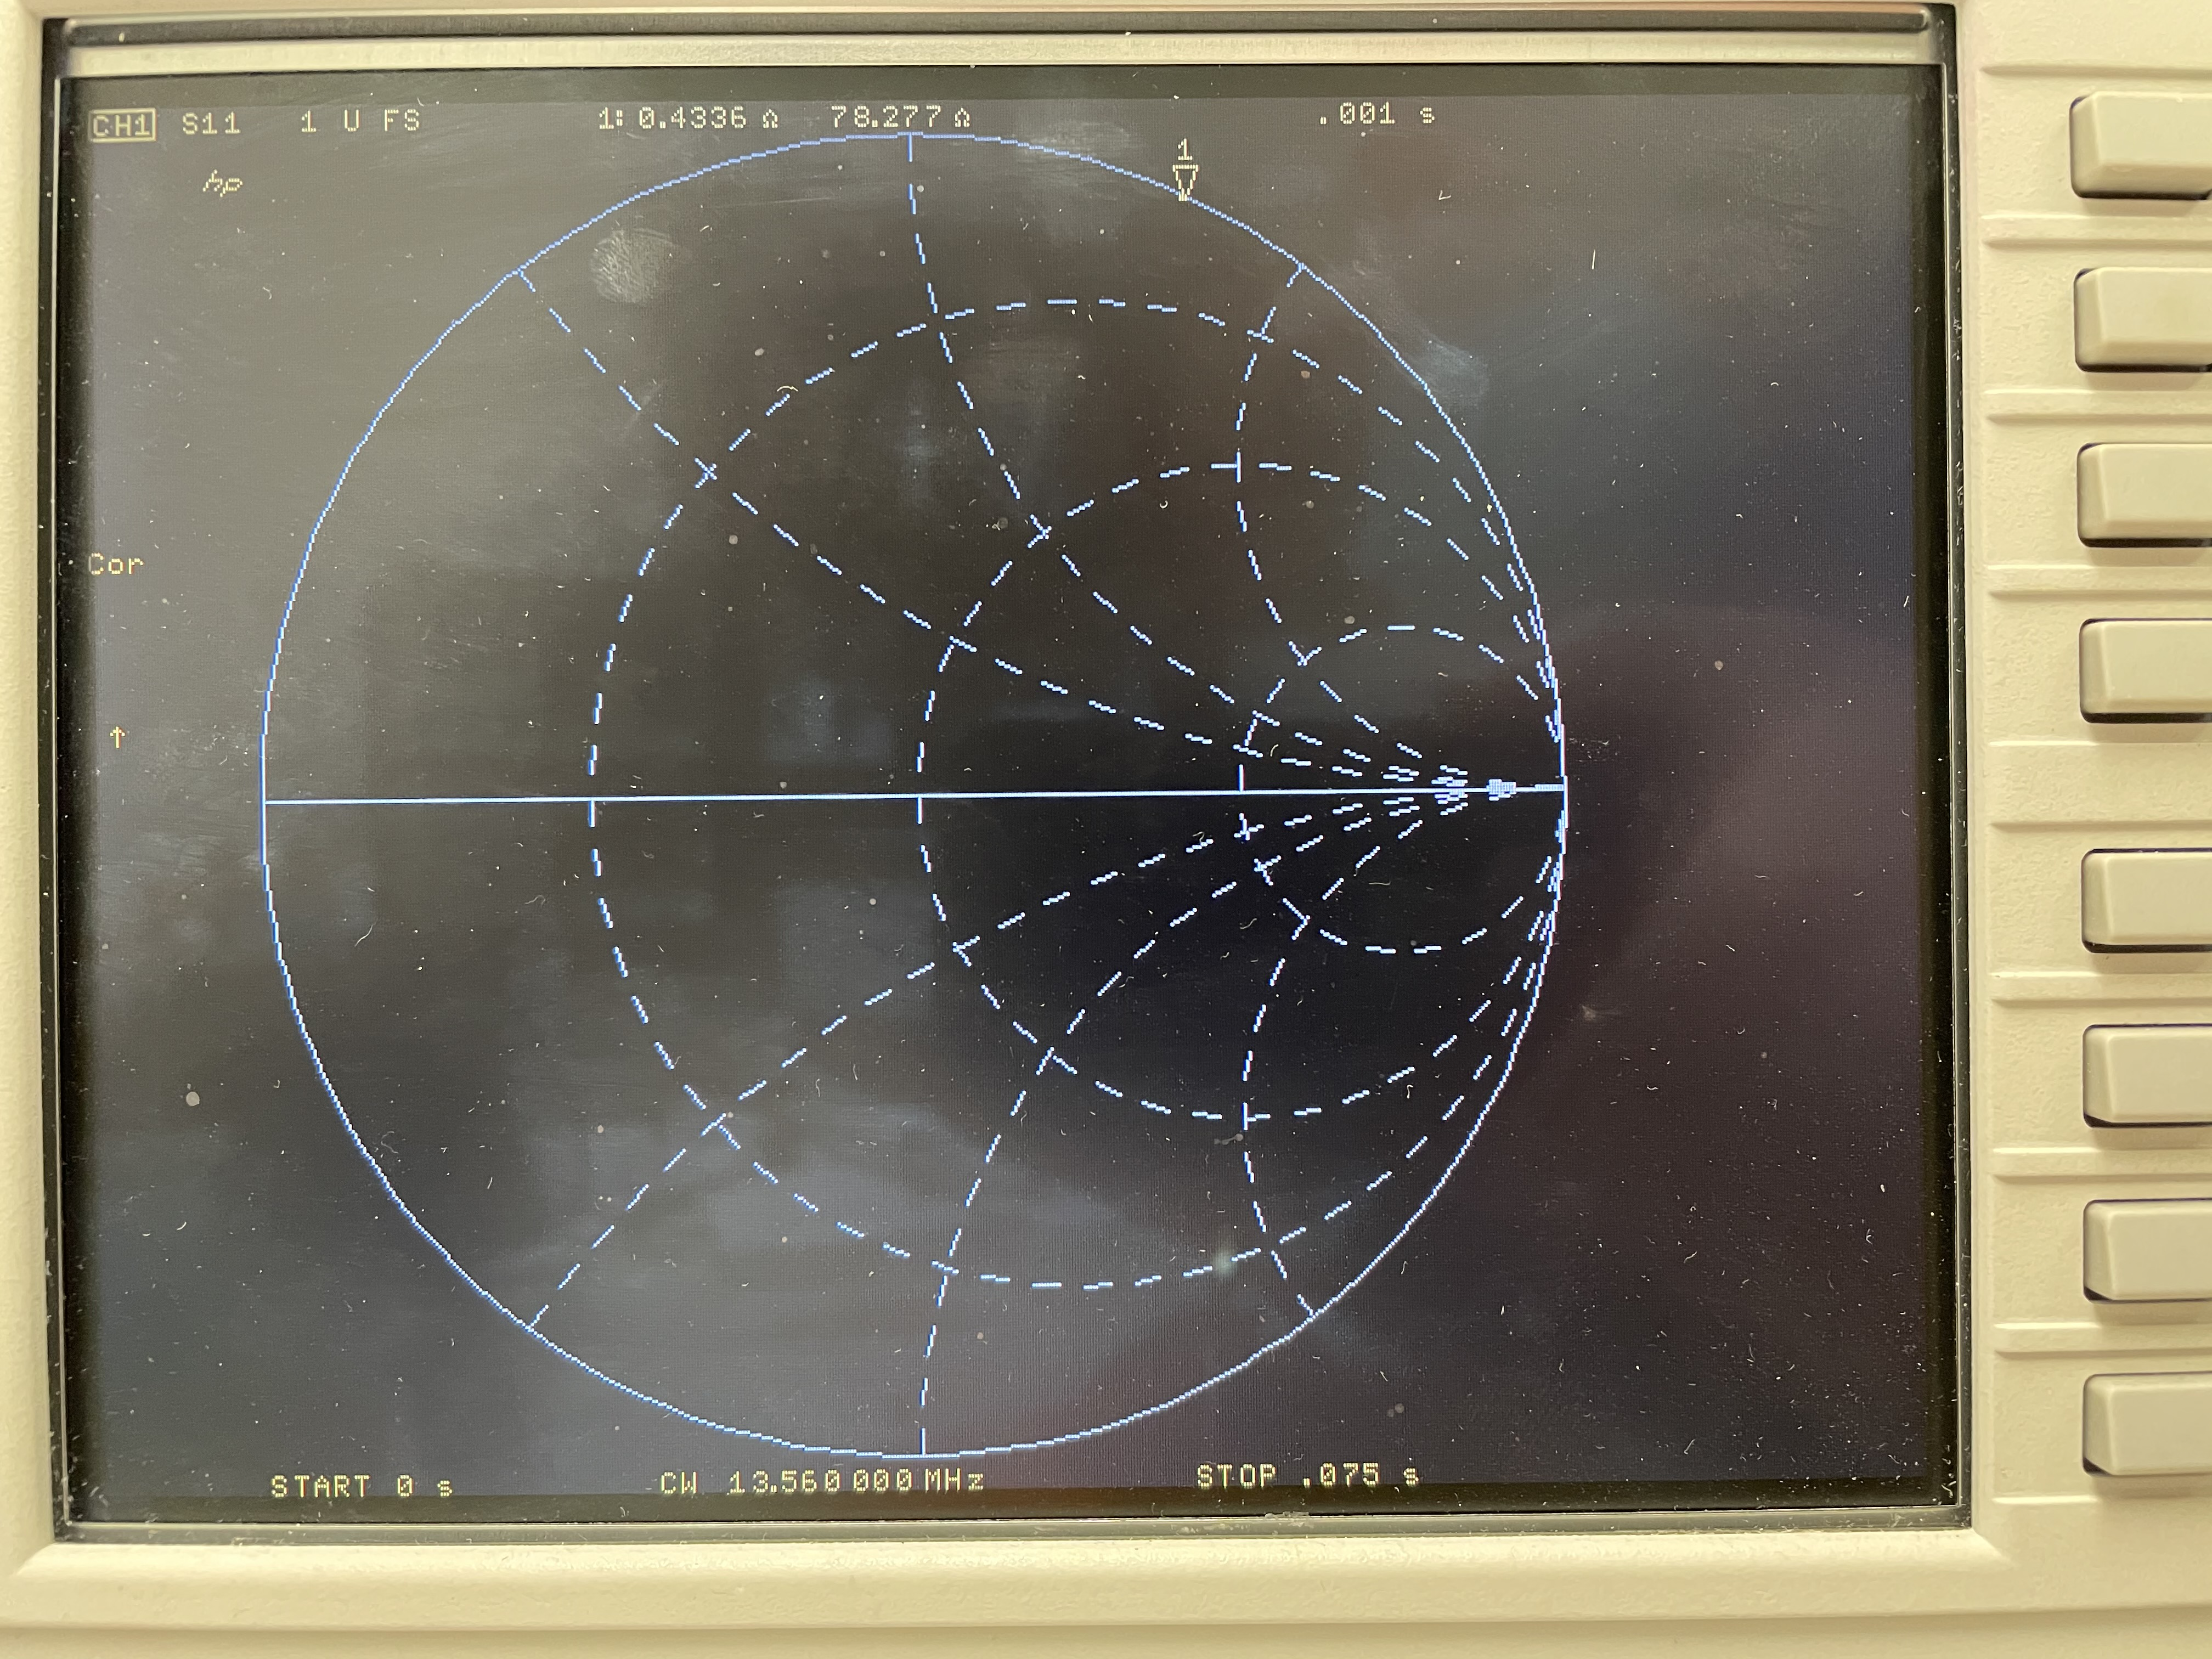
\includegraphics[width=0.8\linewidth]{VNA_measured}
\caption{VNA TX/RX Coil Impedance Measurement}
\end{figure}
\hfill \\
\noindent 
Measured inductance using VNA (HP8753E) 0.917 $\mu$H\\
Measured inductance using LCR meter (HP4262A) 0.97$\mu$H\\
Q factor from VNA impedance measurement: 182
\hfill
\pagebreak
\section{Broader Impacts of the Project}

\indent
This product follows FDA, IEE, and government safety regulations. A few ethical issues faced by our design include high voltages across the coil, excessive heat generation within the receiver, and electromagnetic field interference. During simulation stages, high voltages were observed across the coil which increases the risk of electric shock hazard. In order to lower this risk, the coil insulation will adhere to a wider voltage range. Within the receiver, excessive heat generation along high current levels can cause damage to batteries. Therefore, lower charging currents will be used in order to prevent damage. Excessive heat also increases the cost of the project as fans would need to be added. Electromagnetic field interference caused by the transmitter coil can disrupt the charging circuit and cause battery failure. To prevent this issue, additional shielding will be implemented. \\

\indent
During testing stages, minor ethical issues were faced by the design. Within the receiver board, there was an inductor that was not suited for a frequency of 13.56 MHz board causing failure, and our rectifier circuits caused more loading than expected when tested with a signal generator. Also, the 48V to 30V buck stage microcontroller failed during testing for reasons that are yet to be further investigated by the team. When components get too hot, there’s not only a risk of it failing, but also of leaking its chemicals which can be dangerous to human skin and eyes. Therefore, the group will adhere to safety procedures such as wearing Personal Protective Equipment (PPE). Another risk observed here is electrical shock hazard due to the overloading in the circuit. To prevent this, the group will continuously measure the circuit for abnormal values while testing.\\

\indent
Our project’s goal is to provide users a low-cost medium-power wireless charger. There are no products like this one in the market for a few reasons: chargers do not supply more than 5W via inductive charging, an existing industrial unit with same purposes as our product is priced at about \$2000 USD, and available wireless chargers are limited for charging a single type of device only. With our product, users will be able to charge a standard battery type and integrate it in their own design or use it for stand-alone operations. Our product communicates electronic circuits, electromagnetic fields, digital systems, and microprocessors concepts to the audience. This product will not only be a low-cost wireless charger option, it will also provide customers with a charger for mobile devices of all shapes and sizes, no wiring exposure, apply greater range of tolerance for misalignment when charging, and provide a compact charging area. \\

\indent
Our product will be useful to robotics hobbyists and inventors who are developing new products that require wireless charging, serve to influence kids and teenagers interested in STEM, can be used for research and development, and capitalized in OEM market.

\begin{table}[h!]
\centering
\caption*{Ethical and Professional Considerations}
\begin{tabular} {| r | c | }
\hline
\parbox{0.4\linewidth}{\raggedright Public Health} &   \parbox{0.65\linewidth}{\hfill \\
$\cdot$ Medical Equipment RF Exposure \\ $\cdot$ Electrical Shock \\ $\cdot$ Chemical Exposure}\\
\hline
\parbox{0.4\linewidth}{\raggedright Safety and Wellness} &   \parbox{0.65\linewidth}{\hfill \\
$\cdot$ RF Bandwidth Jamming \\ $\cdot$ Electrical Shock \\ $\cdot$ Chemical Exposure}\\
\hline
\parbox{0.4\linewidth}{\raggedright Global Factors} &   \parbox{0.65\linewidth}{\hfill \\
$\cdot$ International Governing Bodies \\ $\cdot$ Sourcing Restrictions \\ $\cdot$ Inter-Market Penetrability}\\
\hline
\parbox{0.4\linewidth}{\raggedright Societal Factors} &   \parbox{0.65\linewidth}{\hfill \\
$\cdot$ Open-Source Capitalization\\ $\cdot$ STEM Educational Resources \\ $\cdot$ Professional Organizations \\ $\cdot$ Customer Privacy \& Security}\\
\hline
\parbox{0.4\linewidth}{\raggedright Environmental Factors} &   \parbox{0.65\linewidth}{\hfill \\
$\cdot$ Chemical Pollution\\ $\cdot$ User Environmental Awareness\\ $\cdot$ Emergency Shut Off Cases}\\
\hline
\parbox{0.4\linewidth}{\raggedright Economic Factors} &   \parbox{0.65\linewidth}{\hfill \\
$\cdot$ Open-Source Capitalization\\ $\cdot$ Specialty Clientele\\ $\cdot$ Rapid Agile-Deployment\\ $\cdot$ Light-Weight Production}\\
\hline
\end{tabular}
\end{table}
\hfill \\

\section{Conclusion}

\indent
This conclusion reflects the current state of our testing and troubleshooting process. We expect to continue testing our prototype and resolving issues in order to bring performance as close as possible to our initial specifications.\\

\indent
The 5V LCD contrast control circuit on both boards failed due to a design error: the digital potentiometer chosen was not capable of controlling a voltage greater than the 3.3V digital supply voltage. The 5V supplied to the potentiometer simply fed into the 3.3V supply through the protection diodes until the circuit was disabled.\\

\indent
The 48V to 30V buck stage control IC on the transmitter board self-destructed for as-yet unknown reasons. No obvious design errors were found. Further diagnosis was postponed pending testing of the remainder of the board using a bench power supply.\\
\hfill \\
\pagebreak
\hfill \\

\indent
Initial tests of the battery charging circuit were successful. A test battery of two fully charged 18650 cells was correctly detected and not charged further. After partial discharge the charger entered a constant-voltage charging mode and charged the battery at a slowly decreasing current of approximately 1A. The receiver board continued to operate on battery power when simulated wireless power was removed. Further testing of constant current charging, telemetry, and the SMbus smart battery interface is pending.\\

\indent
Initial testing of the wireless power transfer resulted in a period of successful inductive power transfer and a brief success in achieving a resonant link. A failure on the transmitter board was traced to an inductor that was not suitable for operation at 13.56 Mhz. The inductor and damaged components were replaced and testing continued. A resonant link was achieved between the transmitter and receiver, but an unexpected transient destroyed the transmitter amplifier transistor. A more robust replacement will be installed for further testing.\\

\indent
In summation, our testing revealed a few avoidable design errors which can be corrected or managed until a major revision is possible. The greatest challenge our testing has revealed is controlling the high voltages and unexpected transients that even a moderate-power resonant link creates. We hope that the use of more robust components will make it possible to continue testing and characterizing the real-world performance of our wireless power circuit. A further challenge is minimizing the losses from the high-frequency rectification stage. Our initial tests indicate that switching losses in the full wave bridge rectifier are significant. As suggested by our faculty advisor, it is possible that half-wave rectification will prove more efficient than a full-wave bridge.\\

\indent
With the benefit of foresight, we would have made a few minor and one major change in our design process. The wireless power transfer circuit is the most original component of our design and ideally would have been prototyped and tested much earlier in the design process. More minor changes would include accepting the more limited selection of 3.3V LCD’s and deleting the 5V rail and support circuitry. The 48V transmitter power supply and buck stage was chosen to minimize current and provide headroom for adjustments to the wireless transmitter voltage, but further testing may prove that a 30V supply with no further conversion is sufficient.
\hfill 
\pagebreak

%%%%%%%%%%%%%%%%%%%%%%%%%%%%%%%%%%%%%%%%%%%%%%%%%%%%%%%%
%%%%%%%%%%%%%										        %%%%%%%%%%%%%
%%%%						ABOVE IS IN DOCUMENT PROPER					         %%%%
%%%%%%%%%%%%%										        %%%%%%%%%%%%%
%%%%%%%%%%%%%%%%%%%%%%%%%%%%%%%%%%%%%%%%%%%%%%%%%%%%%%%%

%%%% APPENDICES %%%%


%\hline
%\parbox{0.4\linewidth}{\raggedright
%
%} &  \parbox{0.4\linewidth}{\raggedright
%
%}\\
%\hline
\section{Experimental Data Collection Sheets}

\subsection{Transmitter Subsystem Data}

\begin{table}[h!]
\centering
\caption*{Transmitter Subsystem Data}
\begin{tabular}{ | c | c | }
\hline
\textbf{Power Supply Verification} & \textbf{Pass or Fail} \\
\hline
\parbox{0.5\linewidth}{\raggedright \hfill \\[-0.25 em]
30V power supply voltage nominal 30V +/-2\% Measured (TP1) \hfill \\[0.1 em]
} &  \parbox{0.4\linewidth}{\raggedright \hfill \\ [0.7 em]
\underline{\hspace{0.625in}} V  \hspace{0.125 in}Pass \space / \space  Fail \hfill \\ [0.3 em]
} \\
\hline
\parbox{0.5\linewidth}{\raggedright \hfill \\[-0.25 em]
3.3V regulator (U11) test point TP2 nominal voltage 3.3V  tolerance +/- 1.5\% \hfill \\[0.1 em]
} &  \parbox{0.4\linewidth}{\raggedright \hfill \\ [0.7 em]
\underline{\hspace{0.625in}} V  \hspace{0.125 in}Pass \space / \space  Fail \hfill \\ [0.3 em]
} \\
\hline
\parbox{0.5\linewidth}{\raggedright \hfill \\[-0.25 em]
5V regulator (U11) test point TP3 nominal voltage 5V  tolerance +/- 1.5\% \hfill \\[0.1 em]
} &  \parbox{0.4\linewidth}{\raggedright \hfill \\ [0.7 em]
\underline{\hspace{0.625in}} V  \hspace{0.125 in}Pass \space / \space  Fail \hfill \\ [0.3 em]
} \\ 
\hline
\parbox{0.5\linewidth}{\raggedright \hfill \\[-0.25 em]
Coil driver Circuit Test \hfill \\[0.1 em]
} &  \parbox{0.4\linewidth}{\raggedright \hfill \\ [0.7 em]
\underline{\hspace{0.625in}} V  \hspace{0.125 in}Pass \space / \space  Fail \hfill \\ [0.3 em]
} \\ 
\hline
\parbox{0.5\linewidth}{\raggedright \hfill \\[-0.25 em]
Verify functionality of Transmitter Sub-circuits \hfill \\[0.1 em]
} &  \parbox{0.4\linewidth}{\raggedright \hfill \\ [0.7 em]
\underline{\hspace{0.625in}} V  \hspace{0.125 in}Pass \space / \space  Fail \hfill \\ [0.3 em]
} \\ 
\hline
\parbox{0.5\linewidth}{\raggedright \hfill \\[-0.25 em]
Verify Functionality of U11 \hfill \\[0.1 em]
} &  \parbox{0.4\linewidth}{\raggedright \hfill \\ [0.7 em]
\underline{\hspace{0.625in}} V  \hspace{0.125 in}Pass \space / \space  Fail \hfill \\ [0.3 em]
} \\ 
\hline
\parbox{0.5\linewidth}{\raggedright \hfill \\[-0.25 em]
Voltage test for drain of the GaN FET \hfill \\[0.1 em]
} &  \parbox{0.4\linewidth}{\raggedright \hfill \\ [0.7 em]
\underline{\hspace{0.625in}} V  \hspace{0.125 in}Pass \space / \space  Fail \hfill \\ [0.3 em]
} \\ 
\hline
\parbox{0.5\linewidth}{\raggedright \hfill \\[-0.25 em]
Test Peak to Peak Voltage across load \hfill \\[0.1 em]
} &  \parbox{0.4\linewidth}{\raggedright \hfill \\ [0.7 em]
\underline{\hspace{0.625in}} V  \hspace{0.125 in}Pass \space / \space  Fail \hfill \\ [0.3 em]
} \\ 
\hline
\parbox{0.5\linewidth}{\raggedright \hfill \\[-0.25 em]
Test Transmitter Power Output \hfill \\[0.1 em]
} &  \parbox{0.4\linewidth}{\raggedright \hfill \\ [0.7 em]
\underline{\hspace{0.625in}} V  \hspace{0.125 in}Pass \space / \space  Fail \hfill \\ [0.3 em]
} \\ 
\hline
\end{tabular}
\end{table}
\noindent
\textbf{This process is repeated for distances of 5 cm, 4 cm, 3 cm, 2 cm, and 1 cm.}

\subsection{Receiver Regulators Subsystem Data}

\begin{table}[h!]
\centering
\caption*{Receiver Regulators Subsystem Data}
\begin{tabular}{ | c | c | }
\hline
\textbf{Power Supply Verification} & \textbf{Pass or Fail} \\
\hline
\parbox{0.5\linewidth}{\raggedright \hfill \\[-0.25 em]
DC voltage across coil terminals (J2 \& J4)
 \hfill \\[0.1 em]} &  \parbox{0.4\linewidth}{\raggedright \hfill \\ [0.7 em]
\underline{\hspace{0.625in}} V  \hspace{0.125 in}Pass \space / \space  Fail \hfill \\ [0.3 em]
} \\
\hline
\parbox{0.5\linewidth}{\raggedright \hfill \\[-0.25 em]
5V regulator (U11) test point TP3 nominal voltage 5V  tolerance +/- 1.5\%
\hfill \\[0.1 em]} &  \parbox{0.4\linewidth}{\raggedright \hfill \\ [0.7 em]
\underline{\hspace{0.625in}} V  \hspace{0.125 in}Pass \space / \space  Fail \hfill \\ [0.3 em]
} \\
\hline
\parbox{0.5\linewidth}{\raggedright \hfill \\[-0.25 em]
3.3V regulator (U11) test point TP2 nominal voltage 3.3V  tolerance +/- 1.5\%
\hfill \\[0.1 em]} &  \parbox{0.4\linewidth}{\raggedright \hfill \\ [0.7 em]
\underline{\hspace{0.625in}} V  \hspace{0.125 in}Pass \space / \space  Fail \hfill \\ [0.3 em]
} \\ 
\hline
\parbox{0.5\linewidth}{\raggedright \hfill \\[-0.25 em]
Firmware Test Successful Load
\hfill \\[0.1 em]} &  \parbox{0.4\linewidth}{\raggedright \hfill \\ [0.7 em]
\underline{\hspace{0.625in}} V  \hspace{0.125 in}Pass \space / \space  Fail \hfill \\ [0.3 em]
} \\ 
\hline
\end{tabular}
\end{table}
\hfill \\
\pagebreak

\subsection{Receiver Rectifier Subsystem Data}

\begin{table}[h!]
\centering
\caption*{Receiver Rectifier Subsystem Data}
\begin{tabular}{ | c | c | }
\hline
\textbf{Efficiency Test Protocols} & \textbf{Parameters} \\
\hline
\parbox{0.5\linewidth}{\raggedright \hfill \\[-0.25 em]
The transmitter RF output
 \hfill \\[0.1 em]} & 
 30 W\\
\hline
\parbox{0.5\linewidth}{\raggedright \hfill \\[-0.25 em]
The receiver coil placement (parallel)
\hfill \\[0.1 em]} & 
5 cm\\
\hline
\parbox{0.5\linewidth}{\raggedright \hfill \\[-0.25 em]
Current measured
\hfill \\[0.1 em]} &  \parbox{0.4\linewidth}{\raggedright \hfill \\ [0.7 em] \underline{\hspace{0.625in}} 
A 
\hspace{0.125 in}Pass \space / \space  Fail \hfill \\ [0.3 em]} \\ 
\hline
\parbox{0.5\linewidth}{\raggedright \hfill \\[-0.25 em]
Load Voltage measured
\hfill \\[0.1 em]} &  \parbox{0.4\linewidth}{\raggedright \hfill \\ [0.7 em]\underline{\hspace{0.625in}} 
V  
\hspace{0.125 in}Pass \space / \space  Fail \hfill \\ [0.3 em]} \\ 
\hline
\parbox{0.5\linewidth}{\raggedright \hfill \\[-0.25 em]
Load Power
\hfill \\[0.1 em]} &  \parbox{0.4\linewidth}{\raggedright \hfill \\ [0.7 em]\underline{\hspace{0.625in}} 
W
\hspace{0.125 in}Pass \space / \space  Fail \hfill \\ [0.3 em]} \\ 
\hline
\parbox{0.5\linewidth}{\raggedright \hfill \\[-0.25 em]
Efficiency
\hfill \\[0.1 em]} &  \parbox{0.4\linewidth}{\raggedright \hfill \\ [0.7 em]\underline{\hspace{0.625in}} 
\%
\hspace{0.125 in}Pass \space / \space  Fail \hfill \\ [0.3 em]} \\ 
\hline
\end{tabular}
\end{table}
\noindent
\textbf{This process is repeated for distances of 5 cm, 4 cm, 3 cm, 2 cm, and 1 cm.}

\subsection{Charger Subsystem Data}

\begin{table}[h!]
\centering
\caption*{Charger Subsystem Data}
\begin{tabular}{ | c | c | }
\hline
\textbf{Test Protocols} & \textbf{Parameters} \\
\hline
\parbox{0.5\linewidth}{\raggedright \hfill \\[-0.25 em]
Set bench power supply current limit
 \hfill \\[0.1 em]} & 
 1 A \\
\hline
\parbox{0.5\linewidth}{\raggedright \hfill \\[-0.25 em]
Set initial voltage
\hfill \\[0.1 em]} & 
20 V\\
\hline
\parbox{0.5\linewidth}{\raggedright \hfill \\[-0.25 em]
Verify Charger Input Voltage
\hfill \\[0.1 em]} &  
18.6 V\\
\hline
\parbox{0.5\linewidth}{\raggedright \hfill \\[-0.25 em]
Voltage Charger Output
\hfill \\[0.1 em]} &  \parbox{0.4\linewidth}{\raggedright \hfill \\ [0.7 em] \underline{\hspace{0.625in}} 
V 
\hspace{0.125 in}Pass \space / \space  Fail \hfill \\ [0.3 em]} \\ 
\hline
\end{tabular}
\end{table}
\hfill \\
\pagebreak

\subsection{SMBus Subsystem Test  Data}

\begin{table}[h!]
\centering
\caption*{SMBus Subsystem Test Data}
\begin{tabular}{ | c | c | }
\hline
\textbf{Test Protocols} & \textbf{Parameters} \\
\hline
\parbox{0.5\linewidth}{\raggedright \hfill \\[-0.25 em]
Verify Interface Functionality
\hfill \\[0.1 em]} &  \parbox{0.4\linewidth}{\centering \hfill \\ [0.7 em] 
Pass \space / \space  Fail \hfill \\ [0.3 em]} \\ 
\hline
\parbox{0.5\linewidth}{\raggedright \hfill \\[-0.25 em]
Input Undervoltage Setting
\hfill \\[0.1 em]} &  \parbox{0.4\linewidth}{\raggedright \hfill \\ [0.7 em]\underline{\hspace{0.625in}} 
V  
\hspace{0.125 in}Pass \space / \space  Fail \hfill \\ [0.3 em]} \\ 
\hline
\parbox{0.5\linewidth}{\raggedright \hfill \\[-0.25 em]
Final Charge Voltage
\hfill \\[0.1 em]} &  \parbox{0.4\linewidth}{\raggedright \hfill \\ [0.7 em]\underline{\hspace{0.625in}} 
V
\hspace{0.125 in}Pass \space / \space  Fail \hfill \\ [0.3 em]} \\ 
\hline
\parbox{0.5\linewidth}{\raggedright \hfill \\[-0.25 em]
Target Charge Current
\hfill \\[0.1 em]} &  \parbox{0.4\linewidth}{\raggedright \hfill \\ [0.7 em]\underline{\hspace{0.625in}} 
A
\hspace{0.125 in}Pass \space / \space  Fail \hfill \\ [0.3 em]} \\ 
\hline
\parbox{0.5\linewidth}{\raggedright \hfill \\[-0.25 em]
Input Current Limit Target
\hfill \\[0.1 em]} &  \parbox{0.4\linewidth}{\raggedright \hfill \\ [0.7 em]\underline{\hspace{0.625in}} 
A
\hspace{0.125 in}Pass \space / \space  Fail \hfill \\ [0.3 em]} \\ 
\hline
\end{tabular}
\end{table}

\subsection{Coil Subsystem Test Data}
\begin{table}[h!]
\centering
\caption*{Coil Subsystem Test Data}
\begin{tabular}{ | c | c | }
\hline
\textbf{Test Protocols} & \textbf{Parameters} \\
\hline
\parbox{0.5\linewidth}{\raggedright \hfill \\[-0.25 em]
Calibration Test for Short Circuit
\hfill \\[0.1 em]} &  \parbox{0.4\linewidth}{\raggedright \hfill \\ [0.7 em] \underline{\hspace{0.625in}} 
$\mu$H
\hspace{0.125 in}Pass \space / \space  Fail \hfill \\ [0.3 em]} \\ 
\hline
\parbox{0.5\linewidth}{\raggedright \hfill \\[-0.25 em]
Calibration Test for Open Circuit
\hfill \\[0.1 em]} &  \parbox{0.4\linewidth}{\raggedright \hfill \\ [0.7 em]\underline{\hspace{0.625in}} 
$\mu$H
\hspace{0.125 in}Pass \space / \space  Fail \hfill \\ [0.3 em]} \\ 
\hline
\parbox{0.5\linewidth}{\raggedright \hfill \\[-0.25 em]
Calibration Test with 50$\Omega$ Resistive Load
\hfill \\[0.1 em]} &  \parbox{0.4\linewidth}{\raggedright \hfill \\ [0.7 em]\underline{\hspace{0.625in}} 
$\mu$H
\hspace{0.125 in}Pass \space / \space  Fail \hfill \\ [0.3 em]} \\ 
\hline
\parbox{0.5\linewidth}{\raggedright \hfill \\[-0.25 em]
Inductive Reactance
\hfill \\[0.1 em]} &  \parbox{0.4\linewidth}{\raggedright \hfill \\ [0.7 em]\underline{\hspace{0.625in}} 
j$\Omega$
\hspace{0.125 in}Pass \space / \space  Fail \hfill \\ [0.3 em]} \\ 
\hline
\parbox{0.5\linewidth}{\raggedright \hfill \\[-0.25 em]
Impedance
\hfill \\[0.1 em]} &  \parbox{0.4\linewidth}{\raggedright \hfill \\ [0.7 em]\underline{\hspace{0.625in}} 
$\Omega$
\hspace{0.125 in}Pass \space / \space  Fail \hfill \\ [0.3 em]} \\ 
\hline
\parbox{0.5\linewidth}{\raggedright \hfill \\[-0.25 em]
Quality Factor Estimation
\hfill \\[0.1 em]} &  \parbox{0.4\linewidth}{\raggedright \hfill \\ [0.7 em]\underline{\hspace{0.625in}} 
\hspace{0.125 in}Pass \space / \space  Fail \hfill \\ [0.3 em]} \\ 
\hline
\parbox{0.5\linewidth}{\raggedright \hfill \\[-0.25 em]
S$_{21}$ parameter (Forward Voltage Gain)
\hfill \\[0.1 em]} &  \parbox{0.4\linewidth}{\raggedright \hfill \\ [0.7 em]\underline{\hspace{0.625in}} 
\hspace{0.125 in}Pass \space / \space  Fail \hfill \\ [0.3 em]} \\ 
\hline
\end{tabular}
\end{table}


\end{document}
